\documentclass[11pt,a4paper,oneside]{article}
\usepackage[utf8]{inputenc}
\usepackage{amsmath}
\usepackage{amsfonts}
\usepackage{amssymb}
\usepackage{graphicx}
\usepackage{color}
\usepackage {tikz}
\usetikzlibrary {er}
\usepackage[left=2.00cm, right=2.00cm, top=1.00cm]{geometry}
\graphicspath{{./}}

\begin{document}
	\title{DS 256 - Scalable Systems for Data Science \\ Assignment 2}
	\author{Shriram R. \\ M Tech (CDS) \\ 06-02-01-10-51-18-1-15763}
	\maketitle
	
	\section{Introduction}
	Stream Processing has been performed on Twitter Data using Spark Streaming and Kafka. Weak scaling experiments has been conducted for two tasks. The following sections cover the basic summary, experimental setup, plots and analysis.
	
	\section{Basic Summary}
	
	\subsection{ETL Processing}
	This tasks consisted of parsing the twitter JSON objects and extracting different values from it. simple-json library [1] was used to parse JSON. The stop words were added to the program as a static list and was used to normalize the tweet. Each batch of processed tweets was written to individual file. Tweets in which one or more values were missing (Hashtags excluded) were ignored in the output.
	
	\subsection{Hashtag Trends}	
	Processed tweet obtained from the previous task was used to find the trending Hashtags. This task involved a simple map of $<$Hashtag, 1$>$ for each Hashtag and then a reduce step to aggregate the count. The top 5 Hashtags along with their counts were then written to a single file for each batch. The code was tested using a window size of 30s and a slide width of 10s instead of 30min and 10min respectively for brevity.
	
	\subsection{Approximate Distinct Count}
	The Flajolet-Martin algorithm from [2] was implemented to find the approximate distinct counts. 32-bit Murmur hash function from [3] library was used. The algorithm involves parameters like no. of bins, hash functions per bin etc. These are determined as follows:
	\begin{enumerate}
		\item The size (no. of bits) of the hash value was chosen to be 32 since it can fit into an integer and the maximum of no. of distinct users cannot exceed 30 million (less than $2^{32}$) in the given datasets (The full dataset has about 30 million tweets).
		\item The bin size (no. of hashes per bin) was calculated to be 180 which is a small multiple of $log_2m$ where $m$ is the maximum no. of distinct users. This is based on recommendation from [2].
		\item The no. of bins (groups) was set to 15 so as to avoid overestimates and bias. This amounts to 2700 hash computation per row which can be computed in a reasonable time.
	\end{enumerate}


	For all time granularities (hour, day, week) together, each tweet will be processed only once. The aggregates were maintained and reported separately for these granularities. Also, note that the aggregates were reset to 0 for each interval in a given granularity. \\
		
	It was not possible to bound the error induced by approximate count statistically which would have helped to provide a tolerance for the estimate and help in fine tuning the parameters.
		
	\subsection{Sentiment Analysis}
	Sentiment Analysis was performed using the technique provided in [4]. An hashset was built using the keywords and it was intersected with a hashset built from the tweet to find the matching sentiments. One key observation is that there were significant no. of tweets which were not in English language thereby rendering inability to capture the sentiment. The keywords, sentiments and their baselines were statically provided in the code and used.
	     
    \section{Experimental Setup}
    
    \subsection{Hardware}
    Experiments were performed on a commodity cluster having 24 compute nodes. Each node has a 8-core AMD Opteron 3380 processor clocked at 2.6Ghz along with 32GB RAM and 2TB HDD and runs Ubuntu 16.04 LTS (64 bit) with Linux 4.4.0-139-generic. The nodes are connected through a Gigabit Ethernet switch.
    
    \subsection{Apache Kafka}
    Kafka 2.11-2.2.0 was used to stream the twitter data stored in HDFS. Kafka Connect in standalone was used to connect to HDFS. A custom connector was developed to read the files from HDFS and stream them on a given topic. The batch size in Kafka was set to 2000 and delay was varied for different streaming rate. The replication factor was set to 1 for the topic and no. of partitions was varied corresponding to the no. of Spark workers. 
    
    \subsection{HDFS and Apache Spark}
    The cluster is provisioned with Apache Hadoop 3.1.1. HDFS environment has a capacity of 39.54TB with block size 128MB, replication factor of 2 and heartbeat delay of 3s. The global configuration of Spark for all experiments is 4 executor cores per executor (containers) having 8GB of memory. The Driver memory was set to 512MB. Apache YARN was used to coordinate the job execution and jobs were submitted through cluster mode. Experiment specific detail if any is provided below.
       
    \subsection{Dataset}
    
    The dataset used is a collection of 1\% of tweets sampled from Twitter between 17th Oct - 16th Dec 2016. The total dataset size is about 955GB and is stored in HDFS by partitioning the dataset into 3984 files of comparable size (approx. 300MB). Each tweet is described in Twitter Tweet JSON format and is of size approximately 5-10KB . The structure of JSON is described in [5].
    	
    \section{Results \& Analysis}
    
    \subsection{Weak Scaling}
    
    Weak scaling experiments were performed on the ETL and approximate counts task. These two represent different workloads of parsing JSON and computing hash respectively on different set of data. The input stream rate was adjusted depending on the no. of executors to keep the input rate to executor count ratio to be constant. Each experiment was run for approximately 5 minutes and average values are reported below. The Spark batch size was set to 10s for both the tasks. For approx. distinct counting, the granularity was set to 10s, 20s and 30s instead of 1 hour, day and week respectively for brevity.
        
    The plot of time taken by the tasks for each batch of data and speedup versus the executor count is given below,    
    
    \begin{center}
    	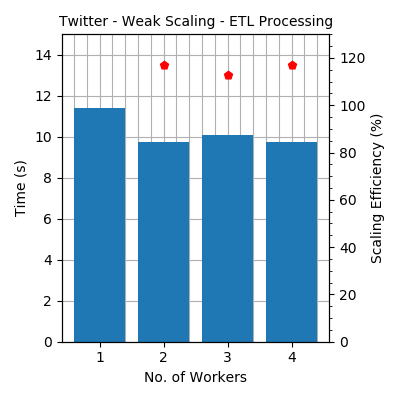
\includegraphics[scale=0.5]{1.png} \\	
    	Figure 1 - Twitter - ETL Processing - Weak Scaling	
    \end{center}

    \begin{center}
    	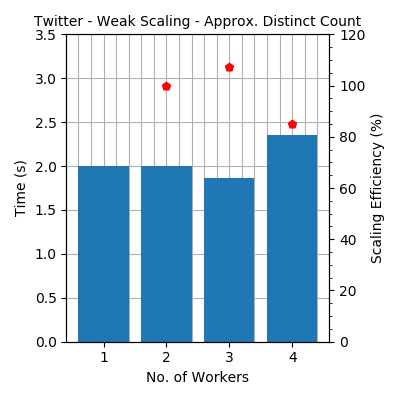
\includegraphics[scale=0.5]{2.png} \\	
    	Figure 2 - Twitter - Approximate Distinct Count - Weak Scaling	
    \end{center}

	It can be observed that Spark Streaming weakly scales for both the tasks. For ETL processing, the speedup is always super-linear whereas both super-linear and linear speedup has been observed for Approximate Distinct count. It must be noted that the processing time is generally less than 10s which is the batching interval in Spark. This is important since of the processing time exceeds 10s, then the latency will start increasing exponentially.
	
	The scheduling delay was observed to be 1-600ms in most of the cases except 1 worker setup for ETL where it was 12s on average and kept increasing due to higher processing time than batching interval (convoy effect).
	
	For Hashtag trending and Sentiment analysis tasks, the processing time taken was in the order of 1s but it is not reported above. Note that, the ETL task took longer time due to JSON parsing and in general the size of input data was large.
	   
   \section{Additional Notes}
   Sample commands to run all the programs with relevant command line arguments is available in the Log file along the Job IDs of all executions. The additional libraries that were used are referenced below. Some idea was taken from the example code introduced in the tutorial.
     
    \section{References}
    \begin{enumerate}{}{}
    	\item https://github.com/fangyidong/json-simple
    	\item Leskovec, Jure, Anand Rajaraman, and Jeffrey David Ullman. Mining of massive datasets. Cambridge university press, 2014.
    	\item https://github.com/google/guava/wiki/HashingExplained
    	\item Sentiment Analysis : ANAS-t: A Psychometric Scale for Measuring Sentiments on Twitter, Pollyanna Goncalves, Fabricio Benevenuto, Meeyoung Cha, SYSTEMS, MAN, AND CYBERNETICS, PART C: APPLICATIONS AND REVIEWS, 2013
    	\item https://developer.twitter.com/en/docs/tweets/data-dictionary/overview/tweet-object.html
    	\item https://www.geeksforgeeks.org/position-of-rightmost-set-bit/
    	\item DS 256 Course Lecture Notes
    	\item https://spark.apache.org/docs/latest/streaming-programming-guide.html
    	\item https://kafka.apache.org/documentation/\#connect
    \end{enumerate}  
    
\end{document}